\chapter{実験}
%評価基準として話を変えないといけない.どちらかというと
\label{chap:evaluation}
\begin{table}[ht]
  \caption{実験環境}
  \label{tab:experiment}
  \centering
  \begin{tabular}{|c|c|} \hline
    ハードウェア & Raspberry Pi 3B+ \\ \hline
    OS & Ubuntu 22.04 LTS \\ \hline
    CPU & 1.4GHz 64-bit quad-core ARM Cortex-A53 \\ \hline
    メモリ & 1GB LPDDR2 SDRAM \\ \hline
    ROS 2 & ROS 2 humble \\ \hline
  \end{tabular}
\end{table}

\begin{table}[ht]
  \centering
  \begin{tabular}{|l|c|c|c|}
  \hline
  /light\_sensors & ROS2 & mROS2 & mROS2-Wasm \\ \hline
  平均値 & 733.40μs & 656.59μs & 2101.89μs \\ \hline
  最大値 & 830μs & 780μs & 2870μs \\ \hline
  最小値 & 650μs & 580μs & 1740μs \\ \hline
  標準偏差 & 58.14μs & 51.16μs & 282.89μs \\ \hline
  \end{tabular}
  \caption{/light\_sensorsの通信時間の統計}
  \label{tab:sensor_stats}
\end{table}

\begin{table}[ht]
  \centering
  \begin{tabular}{|l|c|c|c|}
  \hline
  /cmd\_vel & ROS2 & mROS2-POSIX & mROS2-Wasm \\ \hline
  平均値 & 42757.34μs & 36954.83μs & 46760.56μs \\ \hline
  最大値 & 74220μs & 72490μs & 83190μs \\ \hline
  最小値 & 16550μs & 2380μs & 14170μs \\ \hline
  標準偏差 & 23451.16μs & 20486.34μs & 20424.32μs \\ \hline
  \end{tabular}
  \caption{/cmd\_velの通信時間の統計}
  \label{tab:sensor_stats}
\end{table}

\begin{table}[ht]
  \centering
  \begin{tabular}{|l|c|c|c|}
  \hline
   & ROS2 & mROS2-POSIX & mROS2-Wasm \\ \hline
  RES(Resident Size) & 32.51MB & 1.66MB & 17.37MB \\ \hline
  SHR(Shared Memory) & 25.16MB & 1.48MB & 1,73MB \\ \hline
  RSS(Resident Set Size) & 57.67MB & 3.14MB & 19.10MB \\ \hline
  \end{tabular}
  \caption{各環境の物理消費メモリ(RSS)}
  \label{tab:sensor_stats}
\end{table}

\begin{figure}[ht]
  \centering
  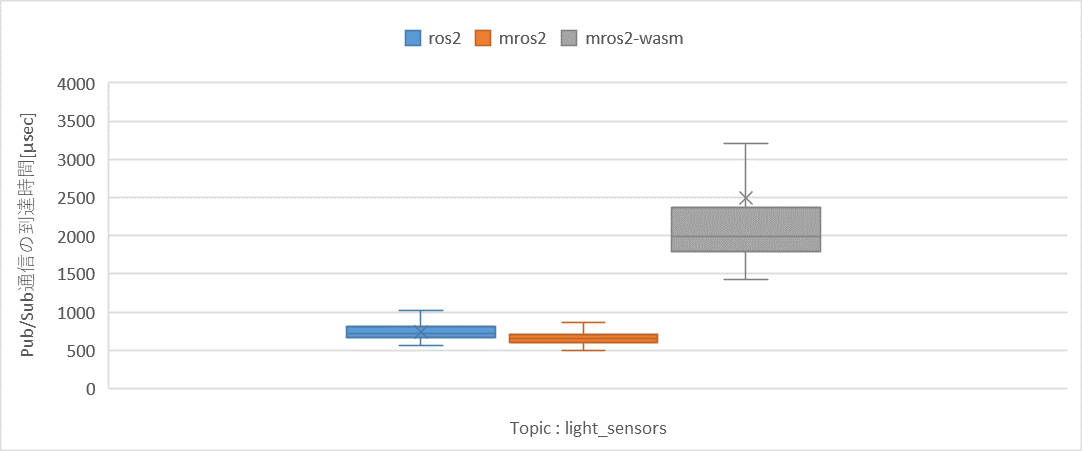
\includegraphics[width=15cm]{images/fig6_lightsensors.png}
  \caption{トピック: /light\_sensorsの通信時間の箱ひげ図}
  \label{fig:light_sensors}
\end{figure}
\begin{figure}[ht]
  \centering
  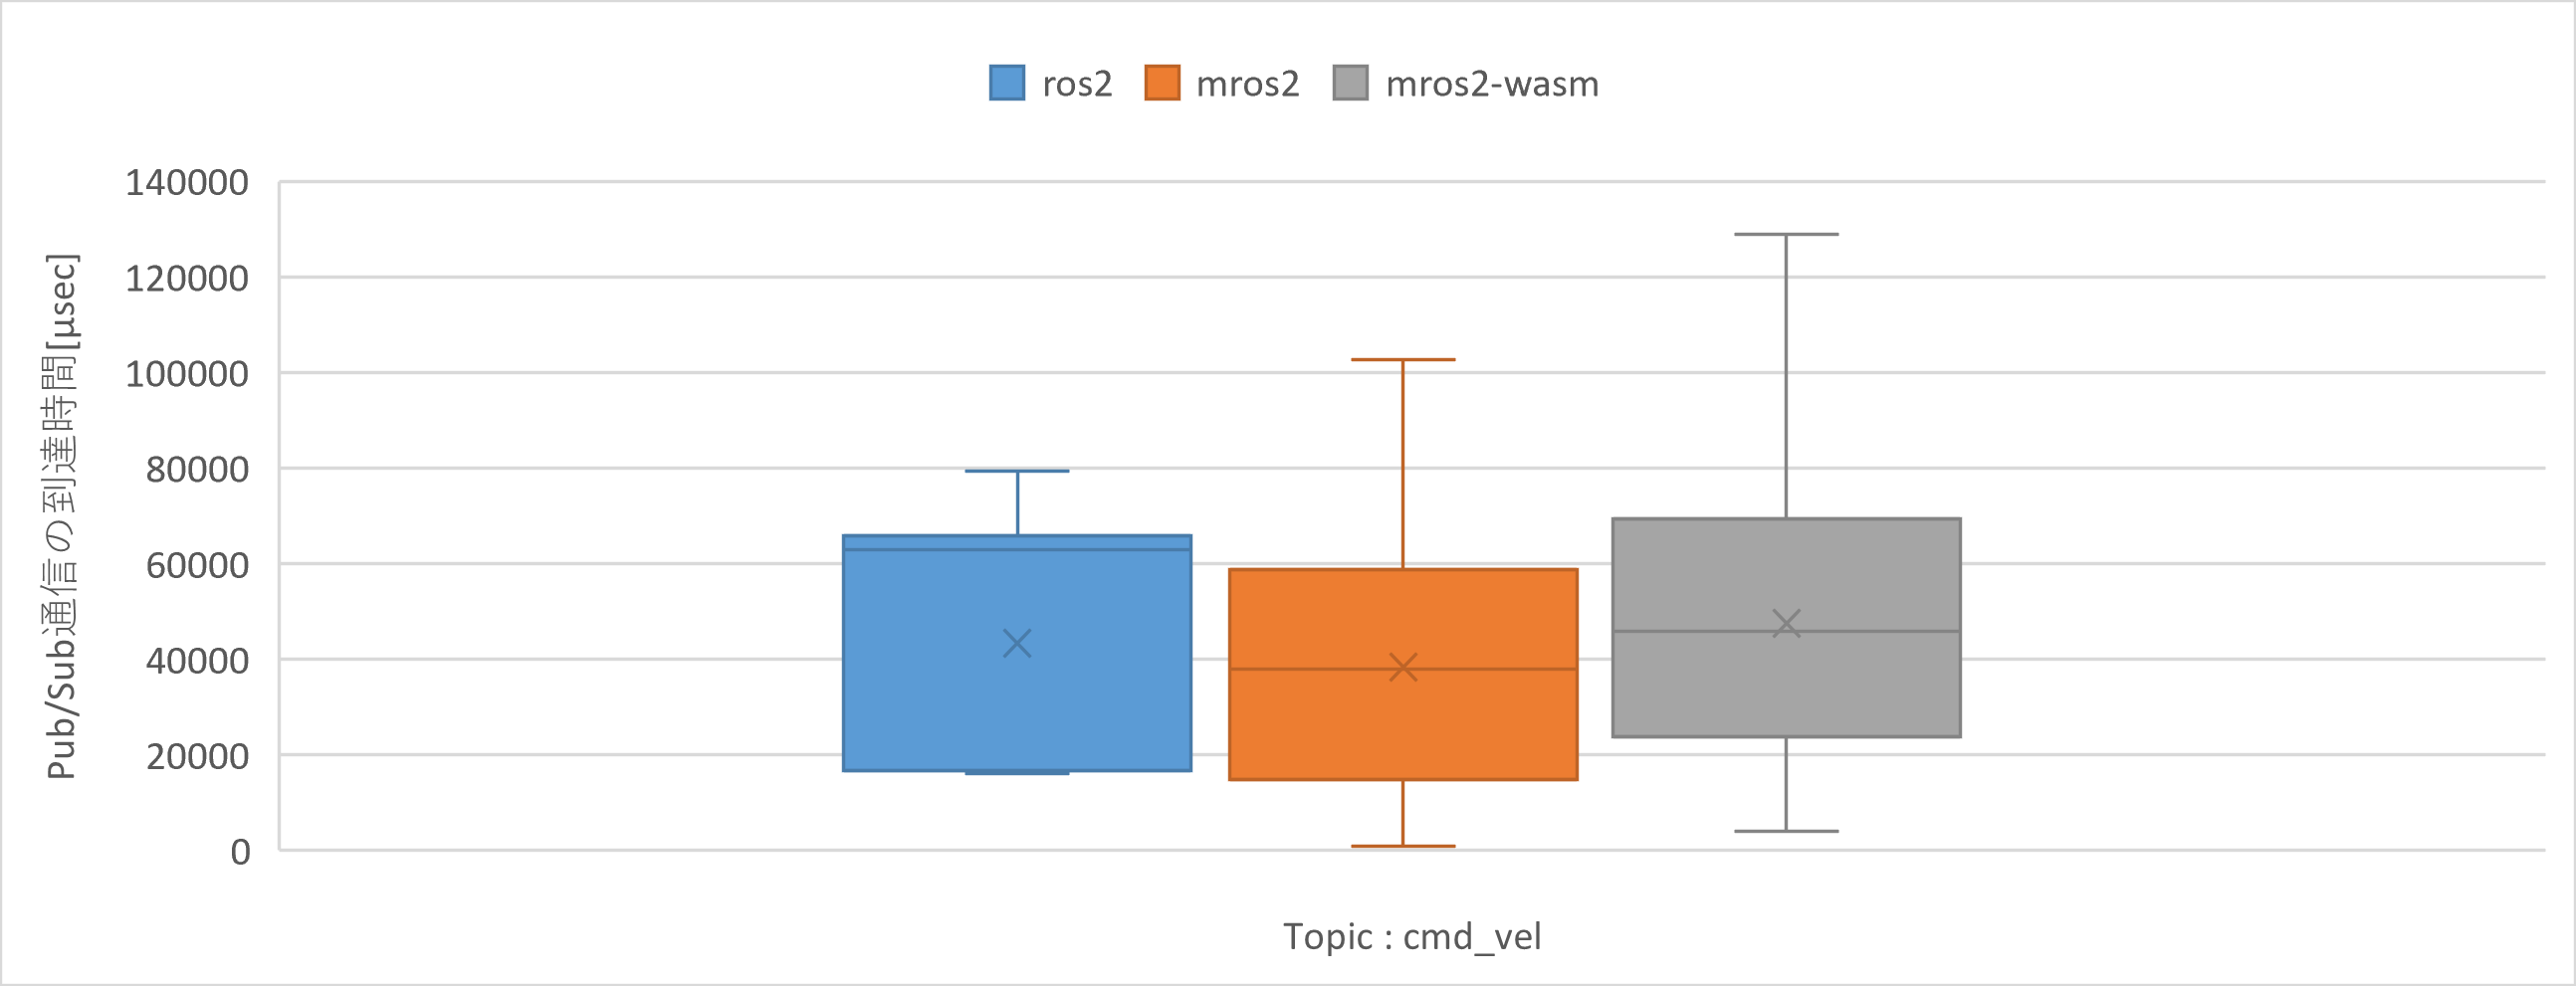
\includegraphics[width=15cm]{images/fig6_cmdvel.png}
  \caption{トピック: /cmd\_velの通信時間の箱ひげ図}
  \label{fig:cmd_vel}
\end{figure}
\begin{figure}[ht]
  \centering
  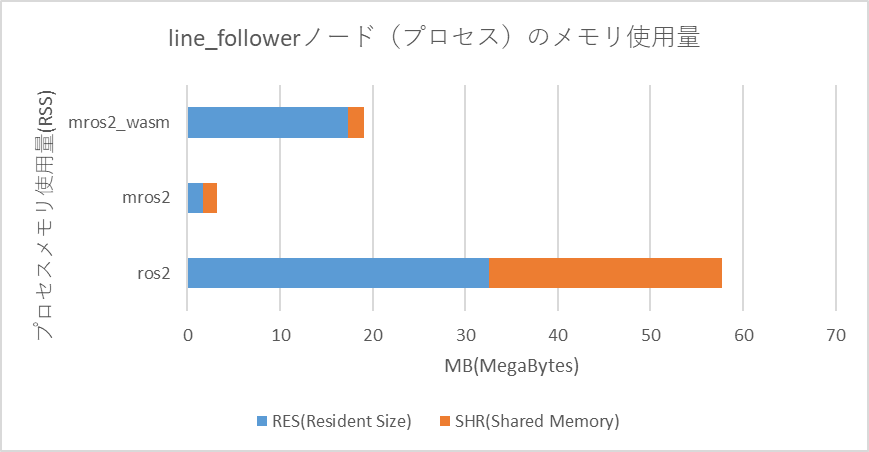
\includegraphics[width=15cm]{images/fig6_mros2-wasm_memory_v2.png}
  \caption{各環境でRES,SHRを合わせたRSSの比較}
  \label{fig:allmemory}
\end{figure}
本章では,実装したアプリケーションを用いて,mROS 2-POSIXとmROS 2-WasmとROS 2の性能を比較評価した実験について述べる.
\section{概要}
本研究でmROS 2-POSIX,mROS 2-Wasm,ROS 2の性能を比較評価するために,それぞれの環境に実装したライントレースノードをラズパイマウスにジョイントしているRassberry Pi 3B+上で動作させ,制御ノードとライントレースノードの通信時間とメモリ消費量を比較する実験を実施した.
\\ 実験の実行環境を表6.1に示す.なお,第2章で述べた通り,ネイティブROS 2のランタイムディストリビューションは最新版であるhumbleを採用した.
\\ 通信時間の計測は,2つのノード間でPub/Sub通信にかかる時間をmROS 2-POSIX,ROS 2間でstd::chrono::high\_resolution\_clockを用いて計測し,mROS 2-Wasm,ROS 2間でLinux標準のclock\_gettime()を用いた.
mROS 2-Wasmでstd::chrono::high\_resolution\_clockを用いると,実行時に取得できる時間がROS 2側のstd::chrono::high\_resolution\_clockと数値が大きく異なり,比較が困難であったためclock\_gettime()を使用した.
時間を計測するトピックは,/light\_sensorsと/cmd\_velである.
このトピックはライントレースする際に使用する主なトピックであり,第4章で述べた通り,/light\_sensorsはライトセンサの値を,/cmd\_velはラズパイマウスのモーターを制御するためのトピックである.
/light\_sensorsはInt16型が4つ格納されている配列であり,/cmd\_velはgeometry\_msgs/Twist型で,float64型が6つ格納されている配列である.
この2つのトピックのPublishした現在時刻,Subscribeした現在時刻を取得し,その差分を通信時間とした.
評価にあたって,通信時間の箱ひげ図,平均値,最大値,最小値,標準偏差を計算した.
/light\_sensorsと/cmd\_velのPub/Subの関係は第5章で述べた通り,/light\_sensorsは制御ノードからPublishされるトピックであり,mROS 2-POSIX,mROS 2-WasmはSubscribeするトピックである.
/cmd\_velはmROS 2-POSIX,mROS 2-WasmがPublishするトピックであり,制御ノードがSubscribeするトピックである.
\\ メモリ消費量の計測は,mROS 2-POSIX,mROS 2-Wasm,ROS 2の各環境でのライントレースノードに対して,実行しているランタイムのプロセスIDを取得し,そのプロセスに割り当てられているRSSを計測した.
各環境で同様の計測を行い,RSSは時間によって変化しなかった.
このRSSを用いて,グラフを作成した.
\section{結果}
実験結果を図6.1から図6.3および表6.2から表6.4に示す.
\\ 図6.1では各環境ごとにトピック/light\_sensorsのPublishした現在時刻とSubscribeした現在時間の差を計算し,箱ひげ図として通信時間のばらつきを示している.
ROS 2とmROS 2-POSIXの通信時間のばらつきは比較的同等であるが,mROS 2-Wasmを見ると,非常に大きなばらつきがあった.
\\ 表6.2は,トピック/light\_sensorsに対して各環境ごとに通信時間の平均値,最大値,最小値,標準偏差を示している.
表6.2を見ると,一番小さい平均値を記録したのがmROS 2-POSIXであり,次いでROS 2,mROS 2-Wasmの順である.
mROS 2-POSIXとROS 2の平均時間の差は約77μsecであり,mROS 2-POSIXとROS 2の通信時間の平均がおおよそ同程度,またはmROS 2-POSIXのPub/Sub通信の方がROS 2よりも若干高速であることだった.
標準偏差は測定値の分布が平均値のまわりにどの程度集まっているか示す指標で小さい順に,mROS 2-POSIX,ROS 2,mROS 2-Wasmの順である.
mROS 2-POSIXとROS 2の差はほとんどなく,若干ROS 2のばらつきが大きいが,ほとんど同程度であった.
mROS 2-Wasmの通信時間の平均がmROS 2-POSIXとROS 2はおおよそ同等であることのに比べて,およそ3倍になっており,標準偏差は,mROS 2-POSIXとROS 2がおおよそ同等であるのに対し,mROS 2-Wasmはおよそ5倍の値になっている.
\\ 図6.2は,図6.1と同様に各環境ごとの/cmd\_velの通信時間のばらつきを示す箱ひげ図である.
図6.2を見ると,mROS 2-POSIXとROS 2とmROS 2-Wasmの通信時間のばらつきはほぼ同等であった.
\\ 表6.3は,表6.2同様トピックの/cmd\_velの通信時間の平均値,最大値,最小値,標準偏差を示している.
表6.3の平均値は,小さい順にmROS 2-POSIX,ROS 2,mROS 2-Wasmの順である.
mROS 2-POSIXとROS 2の差は5082μsecであり,mROS 2-POSIXの方が遅延が少なかった.
また,ROS 2とmROS 2-Wasmの差は4003μsecであり,ROS 2の方が遅延が少なかった.
標準偏差を見ると,小さい順にmROS 2-Wasm,mROS 2-POSIX,ROS 2の順である.
これは平均値の順と逆であり,mROS 2-WasmとmROS 2-POSIXの差はほとんどなく,ROS 2の標準偏差はmROS 2-WasmとmROS 2-POSIXで大きくことなっている.
\\ 図6.3は,ライントレースノードを各環境で動作させたときのRES(Resident Size),SHR(Shared Memory)を合わせたRSSの棒グラフである.
図6.3を見ると,ROS 2とmROS 2-POSIXを比較するとmROS 2-POSIXのほうがメモリ消費量が少なかった.
mROS 2-Wasmのメモリ消費量はROS 2とmROS 2-POSIXと比べて非常に大きな差があった.
\section{考察}
図6.1,表6.2,図6.2,表6.3から,mROS 2-POSIXはROS 2と比べてPub/Sub通信の遅延が少なく,安定かつ高速に通信できていることが分かった.
これは,mROS 2-POSIXが組込み用デバイス向けであるDDSのembeddedRTPSが軽量なTCP/IPスタックであるlwIPを採用しているためだと考える.
さらに,ROS 2とmROS 2-Wasmの通信時間を比べると,ROS 2側がSubscribeを行い,mROS 2-Wasm側がPublishを行うトピック/cmd\_velでは平均の遅延の差は約4000μsecmROS 2-Wasmの遅延が大きかったものの,標準偏差はROS 2よりも小さかった.
しかし,mROS 2-WasmがROS 2からPublishされたメッセージをSubscribeしているトピック/light\_sensorsでは,mROS 2-Wasmの遅延がROS 2の時よりも平均で3倍ほど大きく,標準偏差はおよそ5倍になっていた.これは,mROS 2-WasmがClassicインタプリタでコンパイルされ実行されているのが原因であると考える.しかし,Classicインタプリタで実行されたノードでもPublishの通信時間はROS 2とそこまで大きな差がないということが示された.
\\ 図6.3と表6.4から,mROS 2-POSIXはROS 2と比べてメモリ消費量が少ないということがわかった.これはmROS 2-POSIXがROS 2で実装されているアプリケーションでも軽量なランタイムとして機能しているということを示している.さらに,mROS 2-WasmはROS 2とmROS 2-POSIXと比べて非常に大きなメモリ消費量があった.これはWasm化したことによるオーバーヘッドが大きいため,ROS 2やmROS 2-POSIXと比べて非常に大きな差があったと考える.
